\chapter{Multi-Modal Interaction-Aware Trajectory Optimisation}
\label{text:approach}
In this chapter an overview of the approach is provided. Starting in section \ref{text:approach/formulation} the problem of socially-aware motion planning is formulated formally, including the assumptions made within this project. 
\newline
Section \ref{text:approach/overview} which presents an overview over the full trajectory optimisation pipeline. It is shown how the algorithm is built in order to allow to deal with general graph-like pedestrian behaviour prediction models, with multi-modal, probabilistic outputs. Furthermore, the advantages of formulating socially-aware motion planning as an optimisation problem while utilising graph-based prediction model, e.g. deep learning based models such as the Trajectron \cite{Ivanovic18}, over purely learned \cite{Chen2017} or purely optimisation-based \cite{Berg2011} algorithms are illustrated. Finally it is explained how the usage of a general-purpose, computation-graph based framework such as PyTorch \cite{pytorch} or TensorFlow \cite{tensorflow} can be harnessed for a highly modular, efficient and versatile implementation.
\newline
The exact formulation of the optimisation problem is further explained in section \ref{text:approach/objective} and \ref{text:approach/constraint}. Beginning with the objective function the both the goal-driven and the interaction-driven parts are illustrated, together with a derivation of their gradients. Furthermore, several designs of the specific objective function are discussed. The subsequent section addresses the design of the constraints used. Likewise several constraint function designs are compared. 
\newline
In order to use the system in real-world applications it must comply several requirements. While some of these has been tackled by the optimisation design, e.g. feasibility of the control limitations of the robot or safety regarding robot-human interaction, the system underlies runtime limits. Similarly to \cite{Chen2017} this project aims to run at a frequency of $10 Hz$. To achieve this goal several runtime improvements have been implemented, which are described in section \ref{text:approach/runtime}.


\section{Problem Formulation}
\label{text:approach/formulation}
In this work we are interested in finding the optimal trajectory for a robot navigating among pedestrians on the two-dimensional plane. Let $X_R^t = (x_R^t, y_R^t, vx_R^t, vy_R^t)$ be the position and velocity of the robot, also referred as $ego$, at time $t$ and $X_R$ a trajectory over multiple states $(X_R^{t_0}, X_R^{t_1}, X_R^{t_2}, \hdots, X_R^{T})$. Within this work the robot is assumed to have double integrator dynamics, i.e., 

\begin{align}
\label{eq:robot_dynamics}
\ddot{X}_R^t &= U_R^t. \\
\dot{X}_R^t &= f_R(X_R^t, U_R^t)
\end{align}

For further simplification the robot's dynamics are assumed to be deterministic.
\newline
In general each pedestrian's trajectory is probabilistic and multimodal. Thereby,  let $X_{Pi}^t = \xi_{Pi}^t$ be the state distribution of pedestrian $i$ at time $t$, with mean $\mu_{Pi}^t$, variance $\Sigma_{Pi}^t$ and mode-weights vector $\pi_{Pi}^t$. 

\begin{equation}
X_{Pi}^t = \xi_{Pi}^t \sim f(\mu_{Pi}^t, \Sigma_{Pi}^t, \pi_{Pi}^t)	
\end{equation}

Similar to the robot the pedestrians are modelled as single point masses. The pedestrian's trajectories are predicted using some model $\phi_P$ which is assumed to be known. As described above in general for some pedestrian $P_i$ the model $\phi_P$ outputs a multi-modal distribution over the next state $X_{Pi}^{t+1}$ conditioned on the trajectory of the robot $X_R^{t_0:t}$, the trajectory of every other pedestrian in the scene $X_{Pj}^{t_0:t} (i \neq j)$ and the trajectory of the agent $P_i$ itself, i.e. $X_{Pi}^{t_0:t}$. Moreover the function $\phi_P$ is generally not shared over all pedestrian, but individually for each one.

\begin{equation}
X_{Pi}^{t+1} = \phi_{Pi}(X_R^{t_0:t}, X_{Pi}^{t_0:t}, X_{Pj}^{t_0:t})	
\end{equation}

The set over all pedestrian states over all times within the planning horizon is $\mathcal{S}_P$.
\newline
Furthermore both the robot and the pedestrians underly constraints for their minimal and maximal control effort, $(\mathcal{U}_R^{min}, \mathcal{U}_R^{max})$ and $(\mathcal{U}_P^{min}, \mathcal{U}_P^{max})$ respectively. Thereby all agents are assumed to be isotropic, i.e. have the same boundaries in every dimension.
\newline
Within project \project I want to find a robot trajectory over some discrete time horizon $T$ that trade-offs between minimising the travel time from the its current state to some goal state $\mathcal{G}_R$ on the one side and the interference with the pedestrians in the scene on the other side, with respect to its dynamic as well as safety boundaries. Formally, the solution to this problem solves the following optimisation problem: 

\begin{align}
\min_{U_R} \quad & w_{int} E_{\mathcal{S}_P}[J_{int}(X_R, \mathcal{S}_P)] + w_{goal} J_{goal}(X_R, \mathcal{G}_R) \\
\textrm{s.t. } \quad & X_R^{t+1} = f_R(X_R^t, U_R^t) \\
& X_{Pi}^{t+1} = \phi_{Pi}(X_R^{t_0:t}, X_{Pi}^{t_0:t}, X_{Pj}^{t_0:t}) \\
& g_{control}(X_R) \leq 0 \\
& g_{safety}(X_R, \mathcal{S}_P) \leq 0 \\
\label{eq:formulation}
\end{align} 

For some goal-driven objective function $J_{goal}(\cdot)$ and some interaction-driven objective function $J_{int}(\cdot)$, which are further explained in section \ref{text:approach/objective}; the dynamics for the robot and every pedestrian and some constraint bounding the control effort of the robot $g_{control}(\cdot)$ and ensuring a safe robot-human interaction $g_{safety}(\cdot)$, which will be described in section \ref{text:approach/constraint}.

\section{System Overview}
\label{text:approach/overview}

\begin{figure}[!ht]
\begin{center}

\includegraphics[width=\imgwidth]{images/placeholder.png}
\captionof{figure}{Information-Flow-Diagram of project \project }
\label{img:information_flow}
\end{center}
\end{figure}

- shooting with z = ego controls ($z = U_R$)

- nonzero in equality \& inequality Jacobian, Hessian, number of variables, number of constraints 

- wikipedia description \href{https://en.wikipedia.org/wiki/Trajectory_optimization}{wiki}

- \ac{IPOPT} (fast ! c, cascaded MPC, speed racing)

- Trajectory Optimization (Shooting vs Collocation) \href{https://epubs.siam.org/doi/pdf/10.1137/16M1062569}{tutorial}

- KKT conditions ??

\section{Objective Function Design}
\label{text:approach/objective}

\subsection{Goal Objective}
\label{text:approach/objective/goal}
The goal objective gives an incentive for the optimiser to choose a solution that targets the goal state. It simply consists of the L2-norm between each robot trajectory point and the goal state, normed over the planning horizon:

\begin{equation}
J_{goal}(X_R, \mathcal{G}_R) = \frac{1}{T} \sum_{t = 0}^T (X_R^t - \mathcal{G}_R)^2
\end{equation}

By normalisation the cost is independent from the length of the planning horizon and thus allows to use the same weight $w_{goal}$ for different planning horizons (comp. equation \ref{eq:formulation}). In Figure \ref{img:goal_norm_vs_sum} the convergence of both formulations is compared; although the terminal cost is the same, the normalised version (\textit{goal\_norm}) converges slightly faster, presumably due to the smaller starting value. Although shown for only one scenario here, both, the ease in tuning and slightly larger convergence speed of the normalised goal objective can be observed also over a wide variety of different scenarios.  

\begin{figure}[!ht]
\begin{center}
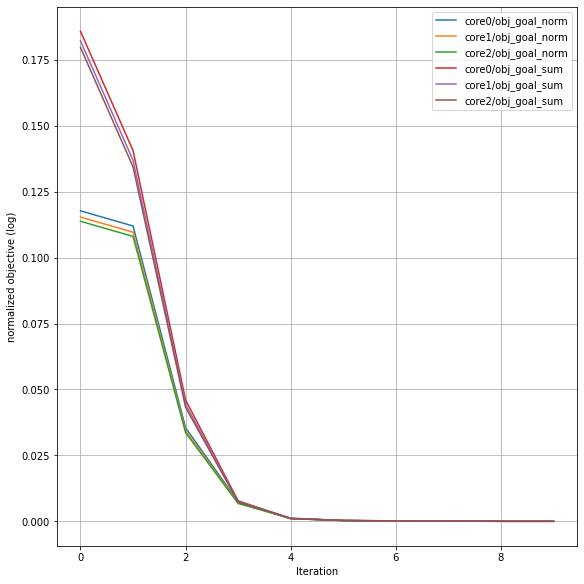
\includegraphics[width=\imgwidth]{images/goal_norm_vs_sum.png}
\captionof{figure}{Direct comparison of a norm-based vs a weighted-sum based goal objective function, normalised by their end value. While roughly the same final objective value is reached (not shown here), the normed goal objective converges faster, i.e. gets to its minimum with fewer iterations over all initial conditions (\textit{core0, core1, core2}). For further details please have a look into the example notebook: \href{https://github.com/simon-schaefer/mantrap/blob/master/examples/modules/goal.ipynb}{examples/modules/goal}.}.
\label{img:goal_norm_vs_sum}
\end{center}
\end{figure}

Since the goal objective $J_{goal}(X_R, \mathcal{G}_R) = J_{goal}(X_R(X_R^0, U_R), \mathcal{G}_R)$ is only a function of the robot's planned trajectory and the goal state, its jacobian can be derived without further knowledge of the pedestrian prediction model, merely using the (known) robot dynamics. As described in section \ref{text:approach/overview} the robot controls are optimised. Hence by applying the chain rule we get: 

\begin{equation}
\nabla J_{goal} = \pd{J_{goal}}{Z} = \pd{J_{goal}}{X_R} \cdot \pd{X_R}{Z}
\end{equation}

Hence, we can find the goal-objectives gradient by determining the gradient of the robot's trajectory with respect to its control inputs and the objectives gradient with respect to the robot's trajectory. Since the goal-objective directly depends on the trajectory, deriving the latter term is trivial: 

\begin{align}
\pd{J_{goal}}{X_R} &= \pd{}{X_R} \frac{1}{T} \sum_{t = 0}^T (X_R^t - \mathcal{G}_R)^2 \\
&= \frac{2}{T} \begin{bmatrix} (X_R^1 - \mathcal{G}_R) X_R^1 & \hdots & (X_R^T - \mathcal{G}_R) X_R^T \end{bmatrix}^T
\end{align}


- jacobian: speed of convergence

- final speed objective

\subsection{Interactive Objective}
\label{text:approach/objective/interactive}

\section{Constraint Function Design}
\label{text:approach/constraint}

\subsection{Control Effort Constraint}
\label{text:approach/constraint/dynamics}

\subsection{Reachability Constraint}
\label{text:approach/constraint/reachability}

however they follow single integrator dynamics. As pointed out in \cite{Ivanovic18} this is an intuitive choice "as a person’s movements are all position-changing, e.g. walking increases position along a direction, running does so faster". Other standard models for pedestrian dynamics such as Social Forces \cite{Helbling1995} however regard the pedestrian to be a double integrator, not a single integrator, and describe the forces acting on it introduced by other pedestrians, obstacles, etc. Having a reasonable fast reaction time and a large maximal acceleration in comparison to the robot both of these descriptions converge, so that the single integrator model is a good choice nonetheless.\footnote{As discussed in chapter \ref{text:experiments} the modular implementation allows to use different pedestrian dynamics. When testing against other prediction environments, in fact, non single integrator dynamics are used, but most analysis described in this report relates to the single integrator model.} 

- constraint formulation (e.g. min-distance constraints split to be more accurate or summed to compute jacobian faster)

- Quellen: neural network representation of value function to make it differentiable (Karen: reachability, Kyle David Julian: network representation to make sure all the corner cases are met)

\section{Runtime Optimisation}
\label{text:approach/runtime}

\subsection{Efficient Trajectory Unrolling}
\label{text:approach/runtime/unrolling}
One of the most promising directions for decreasing the runtime of a trajectory optimisation algorithm is to decrease the runtime of the objective and constraints evaluation as well as their gradients. As shown in sections \ref{text:approach/objective} and \ref{text:approach/constraint} the majority of these optimisation modules depends on the robot's trajectory $X_R$, rather than on its control inputs $U_R$. However since control inputs are optimised, as described in section \ref{text:approach/overview}, a computationally efficient transformation from controls and initial state to the trajectory is key for making the trajectory optimisation real-time feasible.
\newline
Fortunately, we assumed that the robot follows double integrator dynamics, which are linear and markovian. Hence, they can be expressed as the following: 

\begin{equation}
X_R^{t+1} = A X_R^t + B U_R^t
\label{eq:dynamics}
\end{equation}

\begin{minipage}{0.5\textwidth}
$$A = \begin{bmatrix} 1 & 0 & dt & 0 \\ 0 & 1 & 0 & dt \\ 0 & 0 & 1 & 0 \\ 0 & 0 & 0 & 1\end{bmatrix}$$
\end{minipage}
\begin{minipage}{0.5\textwidth}
$$B = \begin{bmatrix} 0 & 0 & dt & 0 \\ 0 & 0 & 0 & dt \end{bmatrix}$$
\end{minipage}

In order to fully "unroll" a trajectory the linear dynamic equation \ref{eq:dynamics} would be to be applied iteratively for the length of the trajectory. Since the dynamics themselves are linear (not just a first-order approximation) this computation can be further batched and on this way, speeded up. In fact the full trajectory can be derived merely based on the initial state $X_R^0$ and the control input matrix $U_R$, as shown in the following:

\begin{align}
X_R^1 &= A X_R^0 + B U_R^0 \\
X_R^2 &= A X_R^0 + B U_R^1 = A^2 X_R^0 + A B U_R^0 + B U_R^1\\ 
\hdots &= \hdots \\
\begin{bmatrix} X^1 \\ X^2 \\ \vdots \\ X^n \end{bmatrix}_R &= \underbrace{\begin{bmatrix} A \\ A^2 \\ \vdots \\ A^n \end{bmatrix}}_{\substack{A_n}} X_R^0 + \underbrace{\begin{bmatrix} B & 0 & \hdots & \hdots & 0 \\ AB & B & 0 & \hdots & 0 \\ \hdots & \hdots & \hdots & \hdots & \hdots \\ A^{n-1} B & A^{n-2} B & \hdots & \hdots & B \end{bmatrix}}_{\substack{B_n}} \begin{bmatrix} U^0 \\ U^1 \\ \vdots \\ U^{n-1}
\end{bmatrix}_R
\end{align}

In summary we get the following (also linear) expression for computing the full robot trajectory at once. As demonstrated in \href{https://github.com/simon-schaefer/mantrap/blob/master/examples/tools/timing.ipynb}{examples/tools/timing} using the fully batched formulation speeds up the trajectory "unrolling" by about a factor of 30.  

\begin{equation}
X_R = A_n X_R^0 + B_n U_R
\label{eq:dynamics_stacked}
\end{equation}

\subsection{Warm Starting}
\label{text:approach/runtime/warm_starting}
It is widely known that warm starting an optimisation can be very beneficial for its convergence speed, e.g. shown in \cite{Banerjee2020} for GuSTO, a sequential convex programming based solver for trajectory optimisation \cite{Bonalli2019}, or for \ac{IPOPT} in \cite{Shahzad2010}, \cite{John2008} or \cite{Spielberge2019}.
\newline
Within project \project the algorithm has been warm-started by solving the optimisation problem posed in equation \ref{eq:formulation} while ignoring all objectives and constraints that relate to pedestrians, i.e. by solving the following optimisation problem: 

\begin{align}
\min_{U_R} \quad & J_{goal}(X_R, \mathcal{G}_R) \\
\textrm{s.t. } \quad & X_R^{t+1} = f_R(X_R^t, U_R^t) \\
& g_{control}(X_R) \leq 0 \\
\label{eq:formulation_warm_starting}
\end{align} 

Since the simplified optimisation problem in equation \ref{eq:formulation_warm_starting} does not depend on the pedestrian dynamics model $\phi_P$ it is much easier and more efficient to solve, being a convex quadratic program. 

\subsection{Agent Filtering}
\label{text:approach/runtime/filtering}

